\chapter{Simulation of Reconstruction Algorithm}
\section{Mathematical Model}
This chapter will describe how the system can be mathematically modeled and how the mask for the lensless imager was chosen. MATLAB has been used for the purpose of simulating the algorithms. A major portion of the MATLAB code for the mathematical model described in this chapter was developed by Ph.D. student Yifeng Shao at Optics Research Group. We present this model to give the reader an idea of the computational algorithm involved in lensless imaging and to understand the work described in the subsequent chapters.
As mentioned in the previous chapter the lensless system can be modelled as,
\begin{equation}
\label{eq:conv2}
I = M * O + e ;
\end{equation}
where $O$ refers to the object scene, $M$ represents the mask function and $I$ represents the image formed on the sensor. We can convert the equation \ref{eq:conv2} to fourier domain and express it as
\begin{equation}
\label{eq:conv3}
F(I) = F(M)F(O)
\end{equation}
\begin{equation}
\label{eq:conv3}
F(O) = \frac{F(I)}{F(M)}
\end{equation}
\begin{equation}
\label{eq:conv4}
O = F^{-1}(\frac{F(I)}{F(M)})
\end{equation}
Equation \ref{eq:conv4} is the simplest possible computational inversion of the scene from the sensor.  However, this method has a limitation of assuming periodic behaviour of object and infinite sensor size. This method cannot be used for imaging extended object scenes with finite sensor sizes. Hence, we need to use other methods to improve our solution and use it for extended object scenes. 
The convolution representation given by equation \ref{eq:conv2} can also be expressed in simple matrix multiplication terms(given by equation \ref{eq:conv5})\cite{Toeplitz}.

\begin{equation}
I1 = M^{''}O1
\label{eq:conv5}
\end{equation} 

where $I1$ and $O1$ are 1-dimensional vectors obtained by concatenating the rows and columns of $I$ and $O$. 
\begin{equation}
I1_{c_I \times i + j} = I_{i, j}
\label{eq:conv6}
\end{equation}

\begin{equation}
O1_{c_O \times i + j} = O_{i,j}
\label{eq:conv7}
\end{equation}
$r_I, c_I, r_O, c_O$ denote the number of rows and columns of the sensor image and the object respectively. The matrix $ M^{''}$ basically has shifted rows of the first row of $ M^{''}$. The first row of $ M^{''}$ is constructed from the mask $M$ by taking each row of $M$, concatenating it with zeros till the vector reaches the size $c_O$. A vector of size $c_O$ is constructed for each row and concatenated together to get the vector for the first row of $ M^{''}$. The matrix $I1$ is a matrix of size $r_Ic_I \times 1$, the matrix  $M^{''}$ is a matrix of size $r_Ic_I \times c_Or_O$ and O1 is matrix of size $c_O r_O \times 1$. The solution is obtained using regularized normal equations:
\begin{equation}
O1_{Guess} = (M^{''T}M^{''} + \alpha^2 1_{r_O \times c_O})^{-1} M^{''T} I1
\label{eq:conv8}
\end{equation}
where $1_{r_O \times c_O}$ represents the identity matrix used for regularizing the equation, remove the zero eigenvalues and make the matrix invertible. The size of the object contributing to the image sensor will be $r_O = r_M + r_I - 1$ and $c_O = c_M + c_I - 1$ pixels. The inversion given by equation \ref{eq:conv8} will take take an extremely long amount of time to solve even using conventional PCs as the inversion can take as long as $10^{18}$ operations for a megapixel image. The number of operations are given by equation \ref{eq:conv9}\cite{Toeplitz}. 

\begin{equation}
N_{Operations} \propto (r_{O}c_{O})^3
\label{eq:conv9}
\end{equation}

Since a generalized mask equation is extremely time-consuming and difficult to solve, separable doubly Toeplitz masks were developed\cite{Toeplitz} to reduce the amount of computation. One main advantage of using this type of mask is that it can be expressed as the outer product of two independent vectors. A separable mask pattern is one in which the mask matrix $M$ can be expressed in terms of a row and column vectors of size $r_M$ and $c_M$ respectively. 
\begin{equation}
M = A(i) B(j)
\label{eq:sepnew_1}
\end{equation}
Both $A$ and $B$ are 1-D vectors. The mathematical model is also changed as described by the equation \ref{eq:sepnew_2}. A non-separable mask is one which does not follow this property. When the mask is separable, equation \ref{eq:conv5} can be simply written as a product of two doubly Toeplitz masks.
\begin{equation}
I = M_A O M_B ^ T
\label{eq:sepnew_2}
\end{equation}

The matrices $M_A$ and $M_B$ are Toeplitz and are of the form given by equation \ref{eq:sepnew_3}.

\begin{equation}
M = 
 \begin{bmatrix*}[r]
    A1 & A2 & \cdots &AN & 0 &0 & \cdots & 0 \\
    0 & A1 & A2 & \cdots &AN & 0 & \cdots & 0\\
    \vdots &\cdots &\cdots &\cdots &\cdots&\cdots&\cdots \\
  \end{bmatrix*}
  \label{eq:sepnew_3}
\end{equation}
The inversions and the multiplication is going to take a lot less time as $r_M$ and $c_M$ are way smaller than $r_O$ and $c_O$ respectively. The number of operations are given by equation \ref{eq:conv9}\cite{Toeplitz}.
\begin{equation}
N_{Operations} \propto (r_{I}c_{O})^3 + (c_{I}c_{O})^3
\label{eq:conv9}
\end{equation}

\begin{table}[ht]
\centering
\caption{Table indicating the rows and columns used for simulation}
\label{tbl:comp_sep}
\begin{tabular}{|c|c|c|}
\hline
Matrix & Rows & Columns \\
\hline
Mask Size, $M$ & $r_M = 1024$ & $c_M = 1024$\\
\hline
Image on Sensor, $I$  & $r_I = 512$ & $c_I = 512$\\
\hline
\makecell{Object Area, $O$ } & \makecell{ $r_O = r_M + r_I - 1$ \\$= 1535$} & \makecell{$c_O = c_M + c_I - 1$\\$ = 1535$}\\
\hline
Left System Vector, $A$ & $r_M = 1024$& 1\\ 
\hline
Right System Vector, $B$ & 1 & $c_M = 1024$\\
\hline
Left Toeplitz Matrix, $M_A$ & $r_{I} = 512$ & $r_{O} = 1535$\\
\hline
Right Toeplitz Matrix, $M_B$ & $c_{I} = 512$ & $c_{O} = 1535$\\
\hline
\end{tabular}
\end{table}
    
\section{Improved Mathematical solution and simulation}
We can improve the solution since a separable mask follows the equation \ref{eq:sepnew_2}. The same improved solution has been used in \cite{Toeplitz}. We can express equation \ref{eq:sepnew_2} as shown in equation \ref{eq:sep_sq}.
\begin{equation}
M_{A}^TIM_{B} = (M_{A}^TM_{A})O(M_{B}^TM_B)^T 
\label{eq:sep_sq}
\end{equation} 
We multiply the left and right system matrices to obtain square symmetric matrices. The problem is that they are not invertible, due to the presence of zero eigenvalues. So, the parameters $\alpha_A$ and $\alpha_B$ are added to remove the zero eigenvalues and make them invertible. The final solution will be given by the equation \ref{eq:sep_final}.
\begin{equation}
O_{Guess} = (M_{A}^TM_A + \alpha_{A}^21_{r_{O}})^{-1}M_{A}^TIM_{B}(M_{B}^TM_B + \alpha_{B}^21_{c_{O}})^{-1}
\label{eq:sep_final}
\end{equation}

The separable mask simulation was carried out as shown in Figure \ref{fig:sep_sim}. We can generate different types of masks by simply changing the base vector that is used for generating $A$ and $B$. We generate $A$ and $B$ by interpolating smaller random vectors. The smaller the random vector, the closer the mask elements. The base vectors are created by generating a random vector of a smaller size(given by simulation variable \texttt{Nxm0} and \texttt{Nym0}) and then setting elements above 0.5 to 1 and elements less than 0.5 to 0. These vectors are interpolated to a larger vector of sizes $r_M \times 1$ and $c_M \times 1$. By simply changing the size of the base vector used for interpolation, we can generate different shapes of Doubly-Toeplitz masks with the same property. In the simulation, the size of the base vector that is used for interpolating to the bigger mask changes. This leads to different masks being generated. The shape of the mask is simpler when we use a smaller vector for interpolation to get a bigger mask. The transmittance of the masks(ratio of open to closed area in the mask) varies between 20 to 25 percent. All the masks offer the same quality of reconstruction in the simulation. The different masks obtained by using different vectors for interpolation is shown in Figure \ref{fig:sep_mask_multi}. The masks generated using vectors of size 16, 32 and 256 is shown in Figure \ref{fig:mask-16}, \ref{fig:mask-32}, \ref{fig:mask-256}. Intuitively, by changing the size of the vector used for interpolation, we can basically change the feature size of the mask. A base vector of smaller size generates a mask where the subsequent binary value comes at a greater distance than the one with a larger base vector.


  \begin{figure}[ht]
    \centering
    \begin{subfigure}{0.5\textwidth}
    \centering
        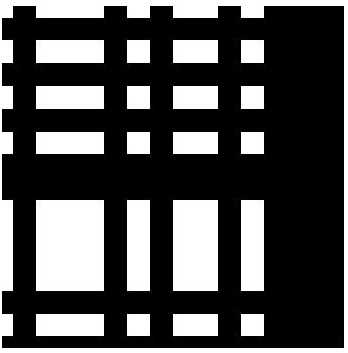
\includegraphics[width=0.5\linewidth]{pics/mask_16}
        \caption{Base Vector of size 16}        
        \label{fig:mask-16}
    \end{subfigure}%
    \begin{subfigure}{0.5\textwidth}
    \centering
        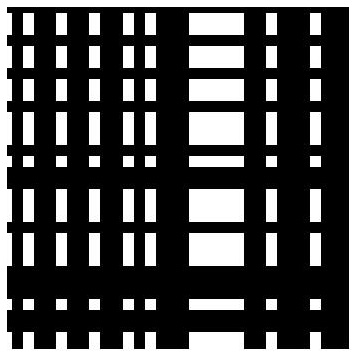
\includegraphics[width=0.5\linewidth]{pics/mask_32}
        \caption{Base Vector of size 32}
        \label{fig:mask-32}
    \end{subfigure}
    
    \begin{subfigure}{0.5\textwidth}
    \centering
        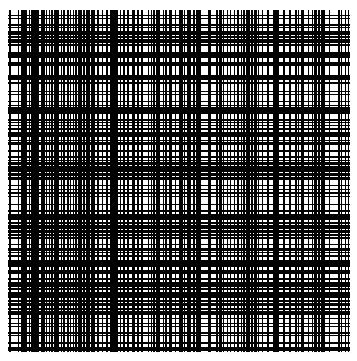
\includegraphics[width=0.5\linewidth]{pics/mask_256}
        \caption{Base Vector of size 256}        
        \label{fig:mask-256}
    \end{subfigure}%     
    \caption{Different separable masks generated by using different vector sizes for interpolation of $A$ and $B$. This produces different masks with the same property but different feature sizes.}
    \label{fig:sep_mask_multi}
    \end{figure}. 
    
In order to start with the mathematical modeling process and to imitate the sensor data and reconstruction, a reference image is needed. For that, it was decided to use the full moon image captured by the Apollo 11 space craft\cite{MoonImage}. Since the satellite is going to be pointing towards astronomical objects like the earth and the moon, it was decided to crop out a portion of the full moon image(See Figure \ref{fig:moon_image}). The simulation is done under the assumption that the camera is enclosed in a box-like structure and light from a specific region of the earth/moon would reach it and the sensor size is finite. The image was converted to gray and scaled down from 0 to 1 and is displayed in the \texttt{bone} colormap format available in MATLAB as the colormap would display the minute variations in the reconstructed image. The mask is then convoluted with the object image(both the mask and image matrices are padded with zeroes to size $r_O \times c_O$). The obtained sensor image is cropped to fit a finite sensor size($r_I \times c_I$). The mask shown in Figure \ref{fig:mask-256} is used for the simulations. 
This is illustrated in Figure \ref{fig:moon_image}. The simulation is performed with and without diffraction effects. The simulation parameters are shown in Table \ref{tbl:sim_parameters}. 

\begin{figure}[ht]
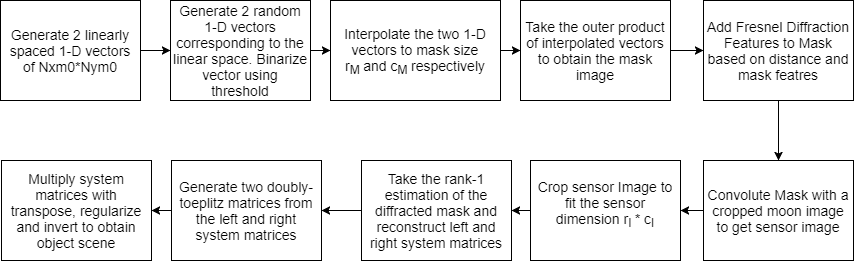
\includegraphics[width=\linewidth]{pics/sep_mask_sim_flow}
\caption{Simulation-Flow separable mask}
\label{fig:sep_sim}
\end{figure}

\begin{figure}[ht]
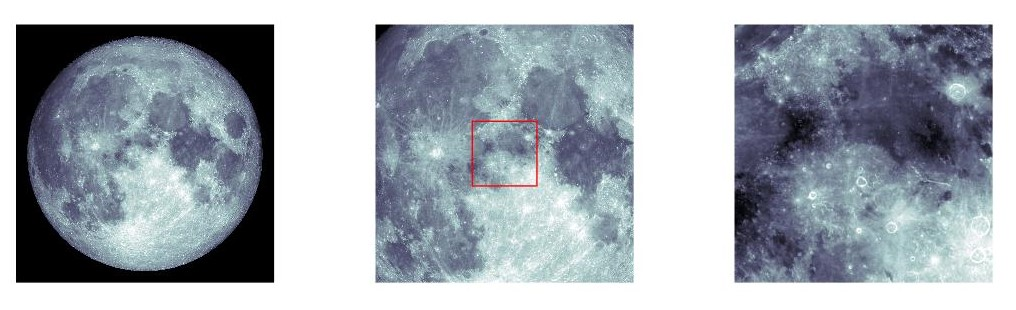
\includegraphics[scale = 0.50]{pics/MoonImagePortion}
\caption{The first image is the original image of the moon as taken by Apollo 11 spacecraft. The second image indicates the cropped region and the third image indicates the region that is used for the simulation.}
\label{fig:moon_image}
\end{figure}

\begin{table}[ht]
\centering
\caption{Simulation Parameters}
\label{tbl:sim_parameters}
\begin{tabular}{|c|c|}
\hline
Pixel Size & 2.2$\mu m$ * 2.2$\mu m$\\
\hline
Sensor Size & 512 * 512 pixels\\
\hline     
Mask Size & 1024 * 1024 pixels\\
\hline 
Mask Sensor Distance & 5 mm \\
\hline 
\end{tabular}
\end{table}

\begin{figure}[ht]
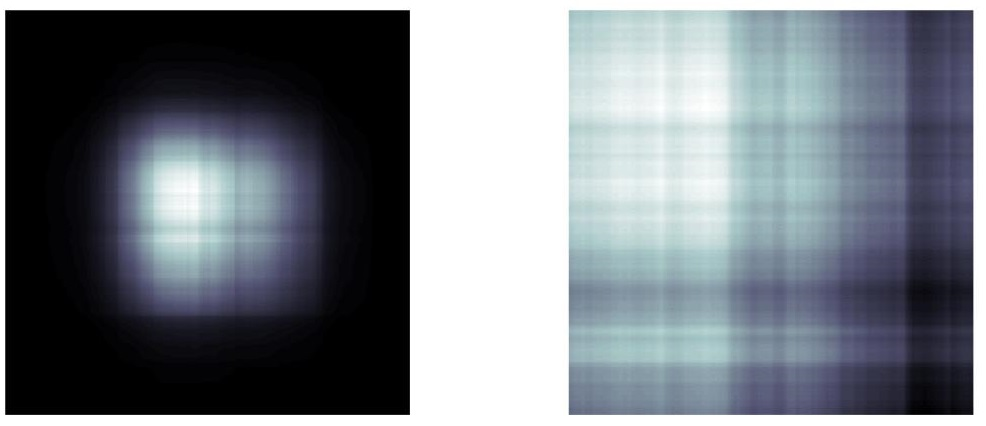
\includegraphics[scale = 0.50]{pics/sensorCropped}
\caption{The first image indicates the sensor image if the sensor plane was infinite. The second image indicates the cropped sensor image that would be formed on an actual finite sensor size(cropped).}
\label{fig:moon_image}
\end{figure}

It can be seen from figure \ref{fig:sep_sim} that there is an additional step apart from the mathematical model involved in the simulation process. It is the rank-1 estimation of diffracted matrices. In this step, we perform Singular Value Decomposition(SVD) on the diffracted matrices to obtain $M_A$ and $M_B$. Now let us see what is singular value decomposition. Singular value decomposition(SVD) is a mathematical tool that would enable us to express any matrix of the form $M_{ m \times n}$ in the form given by equation \ref{eq:svd_1}\cite{svd}. 

\begin{equation}
\label{eq:svd_1}
M_{m \times n} = U_{m \times r}S_{r\times r}(V_{n \times r})^T
\end{equation}
where $r$ represents the rank of the matrix $M$ , $m$ and $n$ denote the size of the matrix respectively. A doubly toeplitz mask in the presence of diffraction effects can be decomposed into $U$ and $V$ which is basically the left and right system vector of the diffracted mask. We can estimate the rank-1 estimation of a matrix by taking the first row and column of $U$ and $V$ and multiplying them as shown in equation \label{eq:svd_2}.

\begin{equation}
\label{eq:svd_2}
M_{1} = U_{1}S_1(V_{1})^T
\end{equation}
One of the main advantages of using a doubly Toeplitz mask is that it is decomposable into a single rank matrix with and without the effects of diffraction. The other rank-components are negligible even in the presence of diffraction. This is an important property that must be kept in mind which will be used for various experimental purposes. Fresnel diffraction features are added to the mask since the distance between the mask and the sensor lies in the Fresnel diffraction region. The Fresnel diffraction modeling is described in the appendix section of the report. Diffraction causes the mask to become non-binary.  In the simulation, we use SVD on the diffracted mask, take the rank-1 estimate of the mask. The $U_1$ and $V_1$ will represent the left and right system matrix of the diffracted mask. The obtained single dimensional $U_1$ and $V_1$ of the diffracted mask will be converted into Toeplitz matrices and inverted using equation \ref{eq:sep_final}. The decomposition of the diffracted and non-diffracted separable mask into a 1-rank matrix(with other components negligible) was also verified in the simulations.
The difference between diffracted and non-diffracted separable mask is shown in Figure \ref{fig:diff_separable}. 

\begin{figure}[ht]
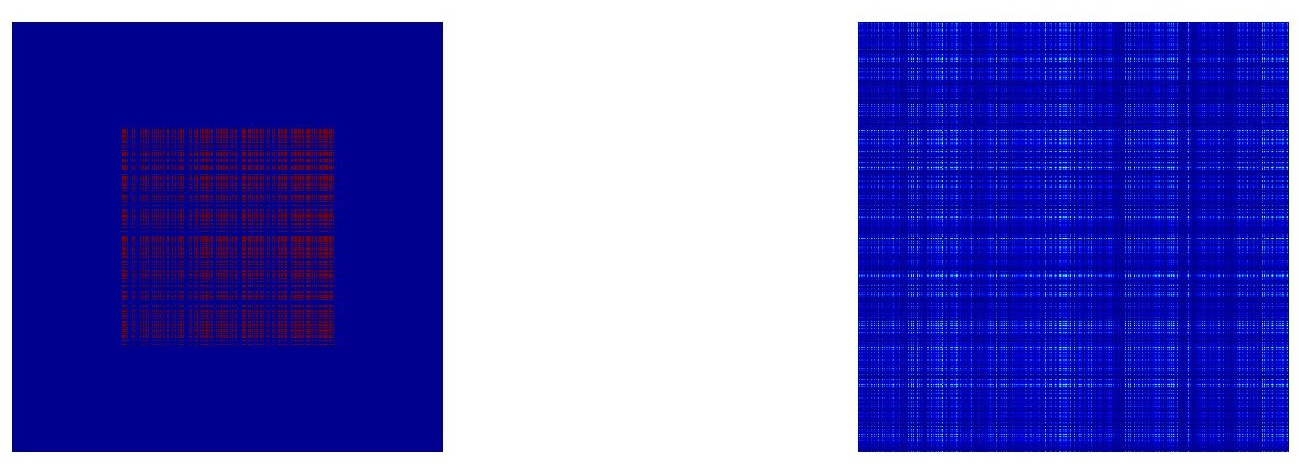
\includegraphics[width=\linewidth]{pics/diffracted_mask}
\caption{The mask on the left indicates undiffracted mask and the mask on the right indicates the diffracted separable mask}
\label{fig:diff_separable}
\end{figure}

The reconstruction error is given by the equation \ref{eq:psnr}.  
\begin{equation}
PSNR = 20log(\frac{N*max(O)}{MSE})
\label{eq:psnr}
\end{equation}
where 
\begin{equation}
MSE = \frac{1}{mn}\sum_{i=1}^{i=N}\sum_{j=1}^{j=N}[O(i,j) - O_{guess}(i,j)]^2
\end{equation}
where $O_{guess}$ indicates the reconstruction and $O$ represents the original object.

It can be seen from Figure \ref{fig:rec_sep} that even in the presence of diffraction it would be possible to obtain reconstructions using equation \ref{eq:sep_final} by using a separable mask. The regularization constants $\alpha_{A}$ and $\alpha_{B}$ were found out by testing for different possible values and the values which gave the best possible reconstruction were chosen.
  \begin{figure}[ht]
    \centering
    \begin{subfigure}{0.5\textwidth}
    \centering
        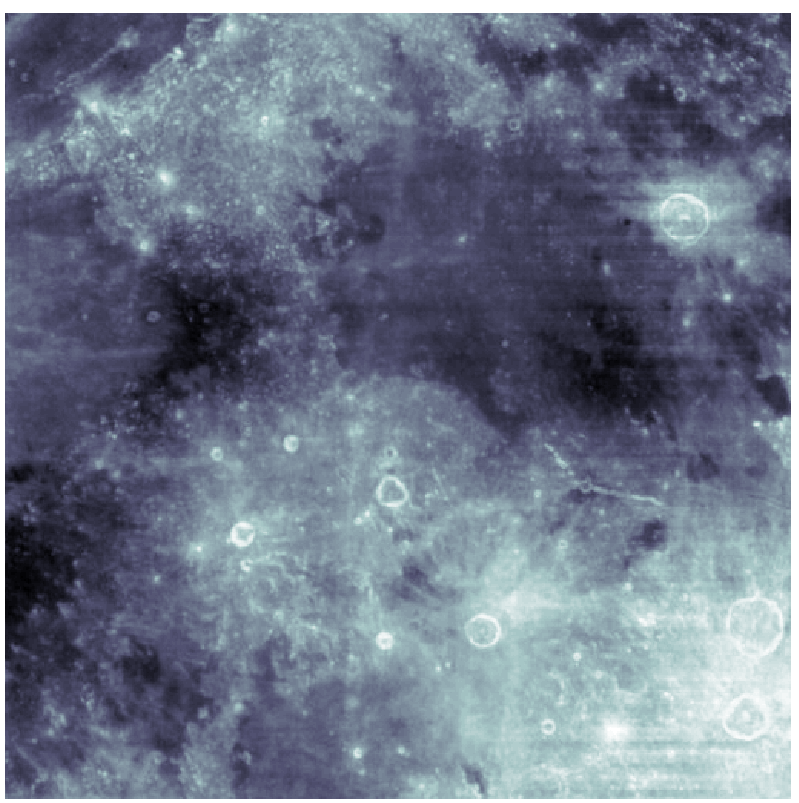
\includegraphics[scale = 0.25]{pics/sep_mask_rec}
    \end{subfigure}%
    \begin{subfigure}{0.5\textwidth}
    \hspace{4cm}    
    \centering
        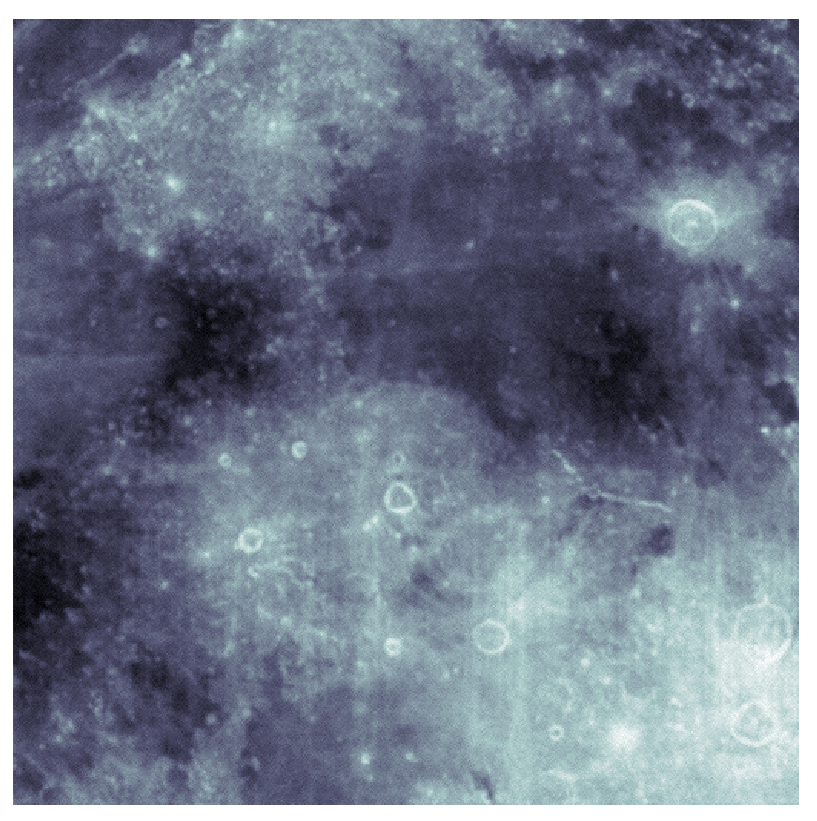
\includegraphics[scale= 0.25]{pics/sep_mask_rec_diff}
    \end{subfigure}
    \caption{The figure shows the reconstruction with and without fresnel diffraction effects for a separable mask using equation \ref{eq:sep_final}. We are able to obtain PSNR = 57.85 without diffraction effects. It can be seen that we can obtain reconstructions even in the presence of diffraction effects with PSNR = 57.93 }
    \label{fig:rec_sep}
    \end{figure}
It was seen that the separable mask would work best for our application and we can safely assume that we can use these masks to obtain reconstructions for extended object imaging in the visible light spectrum as the diffraction effects have also been taken into account.     
   